\documentclass[12pt,a4paper,article]{nsi} % ou eval ou exos ou article
\begin{document}

\titre{Classe NSI}
\classe{2023-09}
\maketitle

\subsection*{changelog}
\begin{itemize}
    \item 2023-09-23 : ajout de l'option \texttt{firamath} qui permet d'utiliser la police Fira Sans Math Light comme police mathématique.
    \item 2023-09-09 : remplacement de la police Source Code Pro par la police Jetbrains pour les passages en code.
    \item 2023-09-08 : ajout de \mintinline{latex}{\reperenb{xmin}{ymin}{xmax}{ymax}{xlabel}{ylabel}}
        \begin{center}
            \begin{tikzpicture}
                \reperenb{-1}{-1}{5}{3}{temps}{revenus (€)}
            \end{tikzpicture}
        \end{center}
    \item 2023-09-07 : changement majeur de l'appel de classe en 1\ere ligne de document.\\
          rectifications et tests.
\end{itemize}


\section*{Options}

\begin{encadrecolore}{Attention}{UGLiRed}
    Désormais les classes \texttt{nsibook}, \texttt{draftnsibook} et autres n'existent plus. Une seule classe est présente : la classe \texttt{nsi}.\\

    Cependant, pour des raisons de rétrocompatibilité, ces anciennes classes sont encore incluses dans le répertoire \texttt{old} mais il est déconseillé de continuer à les utiliser car elles ne sont plus maintenues / mises à jour.
\end{encadrecolore}


Il est possible de passer à la classe toutes les options \textit{traditionnelles} des classes \texttt{book} ou \texttt{article} : \texttt{12pt} ou \texttt{11pt}, \texttt{a4paper} \textit{et cætera}.\\

En plus de ces options traditionnelles
\begin{itemize}
    \item \texttt{cours} sert à fabriquer des chapitres de cours ;
    \item \texttt{exos} sert à fabriquer des feuilles d'exercices ;
    \item \texttt{eval} sert à fabriquer des évaluations ;
    \item \texttt{article} sert à fabriquer de cours documents (ressemble beaucoup à \texttt{exos}).
    \item  l'option \texttt{firamath} permet d'utiliser la police Fira Sans Math Light comme police mathématique.
\end{itemize}
\begin{exemple}[ : création d'une feuille d'exercices]
    \begin{minted}[bgcolor=yellow!10!white]{latex}
        % Anciennement on écrivait
        % \documentclass[12pt,a4paper]{nsiexos} % ou draftnsiexos
        \documentclass[12pt,a4paper,exos]{nsi}
            \classe{\seconde 4}
            \titre{Feuille n°1}
            \begin{document}
                \maketitle
            \end{document}
        \end{minted}
\end{exemple}
Pour tous types de documents, \mintinline{latex}|\maketitle|  utilise \mintinline{latex}{\titre} et \mintinline{latex}{\classe}, sauf \texttt{cours} qui n'utilise pas cette dernière.

\section*{Compilation}

Lorsque le document est compilé avec pdf\LaTeX, la compilation est plus rapide mais les polices de caractères de base sont utilisées.

Avec Lua\LaTeX, la compilation est plus lente mais les polices Fira Sans et Source Code Pro sont chargées.

L'option pdf\LaTeX{} est une bonne manière de préparer le travail, surtout sous Windows car la compilation est très lente.

\section*{Environnements}
\subsection*{Définition}
\begin{minted}[bgcolor=yellow!10!white]{latex}
    \begin{definition}[ : précision]
        contenu
    \end{definition} 
\end{minted}
\begin{definition}[ : précision]
    contenu
\end{definition}
\subsection*{Exemple}
\begin{minted}[bgcolor=yellow!10!white]{latex}
    \begin{exemple}[ : précision]
        contenu
    \end{exemple} 
\end{minted}
\begin{exemple}[ : précision]
    contenu
\end{exemple}
\subsection*{Propriété}
\begin{minted}[bgcolor=yellow!10!white]{latex}
    \begin{propriete}[ : précision]
        contenu
    \end{propriete} 
\end{minted}
\begin{propriete}[ : précision]
    contenu
\end{propriete}
\subsection*{Notation}
\begin{minted}[bgcolor=yellow!10!white]{latex}
    \begin{notation}[ : précision]
        contenu
    \end{notation} 
\end{minted}
\begin{notation}[ : précision]
    contenu
\end{notation}
\subsection*{Méthode}
\begin{minted}[bgcolor=yellow!10!white]{latex}
    \begin{methode}[ : précision]
        contenu
    \end{methode} 
\end{minted}
\begin{methode}[ : précision]
    contenu
\end{methode}
\subsection*{Remarque}
\begin{minted}[bgcolor=yellow!10!white]{latex}
    \begin{remarque}[ : précision]
        contenu
    \end{remarque} 
\end{minted}
\begin{remarque}[ : précision]
    contenu
\end{remarque}
\subsection*{À retenir}
\begin{minted}[bgcolor=yellow!10!white]{latex}
    \begin{aretenir}[ : précision]
        contenu
    \end{aretenir} 
\end{minted}
\begin{aretenir}[ : précision]
    contenu
\end{aretenir}

\subsection*{Pour le code}
\begin{minted}[bgcolor=yellow!10!white]{latex}
\begin{pyc}
    \begin{minted}{python}
        def f(x: float) -> float:
            return 0.5 * x ** 2
    end{minted} % avec un \ devant
end{pyc}% avec un \ devant
\end{minted}
\begin{pyc}
    \begin{minted}{python}
        def f(x: float) -> float:
            return 0.5 * x ** 2
    \end{minted}
\end{pyc}

\begin{minted}[bgcolor=yellow!10!white]{latex}
    Je veux vous parler de la fonction \mintinline{python}{print} de \textsc{Python}. 
\end{minted}
Je veux vous parler de la fonction \mintinline{python}{print} de \textsc{Python}.


\subsection*{Encadré coloré custom}

\begin{minted}[bgcolor=yellow!10!white]{latex}
    \begin{encadrecolore}{Titre customisé de la couleur désirée}{UGLiDarkBlue}
        contenu
    \end{encadrecolore}
\end{minted}
\begin{encadrecolore}{Titre customisé de la couleur désirée}{UGLiDarkBlue}
    contenu
\end{encadrecolore}

\section*{Environnements énumératifs}
\subsection*{Liste ordonnée}
\begin{minted}[bgcolor=yellow!10!white]{latex}
\begin{enumerate}
    \item truc ;
    \item machin ;
    \item bidule.
\end{enumerate}
\end{minted}
\begin{enumerate}
    \item truc ;
    \item machin ;
    \item bidule
\end{enumerate}

\subsection*{Liste non ordonnée}
\begin{minted}[bgcolor=yellow!10!white]{latex}
\begin{itemize}
    \item truc ;
    \item machin ;
    \item bidule.
\end{itemize}
\end{minted}

\begin{itemize}
    \item truc ;
    \item machin ;
    \item bidule.
\end{itemize}

\subsection*{QCM}
\begin{minted}[bgcolor=yellow!10!white]{latex}
Une question à choix multiples
\begin{qcm}
    \item Réponse 1
    \item Réponse 2
    \item Réponse 3
\end{qcm}
\end{minted}
Une question à choix multiples
\begin{qcm}
    \item Réponse 1
    \item Réponse 2
    \item Réponse 3
\end{qcm}

\section*{Couleurs}
\begin{minted}[bgcolor=yellow!10!white]{latex}
    \color{UGLiPurple} UGLiPurple \\
    \color{UGLiRed} UGLiRed \\
    \color{UGLiOrange} UGLiOrange \\
    \color{UGLiYellow} UGLiYellow \\
    \color{UGLiGreen} UGLiGreen \\
    \color{UGLiDarkGreen} UGLiDarkGreen \\
    \color{UGLiBlue} UGLiBlue \\
    \color{UGLiDarkBlue} UGLiDarkBlue 
\end{minted}
\color{UGLiPurple} UGLiPurple \\
\color{UGLiRed} UGLiRed \\
\color{UGLiOrange} UGLiOrange \\
\color{UGLiYellow} UGLiYellow \\
\color{UGLiGreen} UGLiGreen \\
\color{UGLiDarkGreen} UGLiDarkGreen \\
\color{UGLiBlue} UGLiBlue \\
\color{UGLiDarkBlue} UGLiDarkBlue \color{black}

\section*{Tables}

Le style de table par défaut est selectionnable avec \mintinline{latex}{\tabdefaut} (ou \mintinline{latex}{\tabulardefaut} pour rétrocompatibilité).

\begin{minted}[bgcolor=yellow!10!white]{latex}
\tabdefault
\begin{tabular}{|c|c|c|}
    \hline
    Colonne 1 & Colonne 2 & Colonne 3 \\\hline
    Valeur 1  & Valeur 2  & Valeur 3  \\\hline
    Valeur 4  & Valeur 5  & Valeur 6  \\\hline
    Valeur 7  & Valeur 8  & Valeur 9  \\\hline
    Valeur 10 & Valeur 11 & Valeur 12 \\\hline
    Valeur 13 & Valeur 14 & Valeur 15 \\\hline
\end{tabular}
\end{minted}
\tabdefault
\begin{tabular}{|c|c|c|}
    \hline
    Colonne 1 & Colonne 2 & Colonne 3 \\\hline
    Valeur 1  & Valeur 2  & Valeur 3  \\\hline
    Valeur 4  & Valeur 5  & Valeur 6  \\\hline
    Valeur 7  & Valeur 8  & Valeur 9  \\\hline
    Valeur 10 & Valeur 11 & Valeur 12 \\\hline
    Valeur 13 & Valeur 14 & Valeur 15 \\\hline
\end{tabular}\\

On peut styler les tables avec \mintinline{latex}{\tabstyle[couleur]} (ou \mintinline{latex}{\tabularstyle[couleur]} pour rétrocompatibilité)

\begin{minted}[bgcolor=yellow!10!white]{latex}
    \tabstyle[UGLiGreen]
    \begin{tabular}{|c|c|c|}
        \hline
        Colonne 1 & Colonne 2 & Colonne 3 \\\hline
        Valeur 1  & Valeur 2  & Valeur 3  \\\hline
        Valeur 4  & Valeur 5  & Valeur 6  \\\hline
        Valeur 7  & Valeur 8  & Valeur 9  \\\hline
        Valeur 10 & Valeur 11 & Valeur 12 \\\hline
        Valeur 13 & Valeur 14 & Valeur 15 \\\hline
    \end{tabular}
    \end{minted}
\tabstyle[UGLiGreen]
\begin{tabular}{|c|c|c|}
    \hline
    Colonne 1 & Colonne 2 & Colonne 3 \\\hline
    Valeur 1  & Valeur 2  & Valeur 3  \\\hline
    Valeur 4  & Valeur 5  & Valeur 6  \\\hline
    Valeur 7  & Valeur 8  & Valeur 9  \\\hline
    Valeur 10 & Valeur 11 & Valeur 12 \\\hline
    Valeur 13 & Valeur 14 & Valeur 15 \\\hline
\end{tabular}\\

\`A l'intérieur d'un tableau stylé on peut utiliser la commande \mintinline{latex}{\ccell} ( ou \mintinline{latex}{\ths} pour rétrocompatibilité) pour obtenir une cellule d'en-tête.
Pour une cellule blanche, utiliser \mintinline{latex}{\bcell}


\begin{minted}[bgcolor=yellow!10!white,fontsize=\small]{latex}
    \tabstyle[UGLiOrange]
    \begin{tabular}{|c|c|c|}
        \hline
        \bcell           & \ccell Colonne 2 & \ccell Colonne 3  \\\hline
        \ccell Valeur 1  & Valeur 2         & Valeur 3          \\\hline
        \ccell Valeur 4  & Valeur 5         & Valeur 6          \\\hline
        \ccell Valeur 7  & Valeur 8         & Valeur 9          \\\hline
    \end{tabular}
    \end{minted}
\tabstyle[UGLiGreen]
\tabstyle[UGLiOrange]
\begin{tabular}{|c|c|c|}
    \hline
    \bcell          & \ccell Colonne 2 & \ccell Colonne 3 \\\hline
    \ccell Valeur 1 & Valeur 2         & Valeur 3         \\\hline
    \ccell Valeur 4 & Valeur 5         & Valeur 6         \\\hline
    \ccell Valeur 7 & Valeur 8         & Valeur 9         \\\hline
\end{tabular}\\

Lors de l'insertion d'une table dans un environnement, si le style des tables n'est pas \mintinline{latex}{\tabdefaut}, les couleurs de la table suivent celles de l'environnement :
\begin{minted}[bgcolor=yellow!10!white,fontsize=\small]{latex}
    \begin{exemple}[]
        \begin{tabular}{|c|c|c|}
            \hline
            \bcell           & \ccell Colonne 2 & \ccell Colonne 3  \\\hline
            \ccell Valeur 1  & Valeur 2         & Valeur 3          \\\hline
            \ccell Valeur 4  & Valeur 5         & Valeur 6          \\\hline
            \ccell Valeur 7  & Valeur 8         & Valeur 9          \\\hline
        \end{tabular}        
    \end{exemple}   
\end{minted}
\begin{exemple}[]
    \begin{tabular}{|c|c|c|}
        \hline
        \bcell          & \ccell Colonne 2 & \ccell Colonne 3 \\\hline
        \ccell Valeur 1 & Valeur 2         & Valeur 3         \\\hline
        \ccell Valeur 4 & Valeur 5         & Valeur 6         \\\hline
        \ccell Valeur 7 & Valeur 8         & Valeur 9         \\\hline
    \end{tabular}
\end{exemple}

\section*{Mise en page}

Avec les commandes
\begin{itemize}
    \item \mintinline{latex}{\picleft{fraction}{fichier}{texte}} ( ou \mintinline{latex}{\floatpictureleft} pour rétrocompatibilité) ;
    \item \mintinline{latex}{\picleftc{fraction}{fichier}{legende}{texte}} ( ou \mintinline{latex}{\floatpictureleftcaption} pour rétrocompatibilité) ;
    \item Même chose à droite.
\end{itemize}
\begin{minted}[bgcolor=yellow!10!white]{latex}
    Du texte avant.\\
    \picleft{0.3}{iris.png}{
        Une image à gauche avec du texte à droite. En général on s'arrange pour que le premier paramètre, qui est la fraction de la largeur de la ligne occupée par l'image et la quantité de texte à droite soient en harmonie sinon voici ce que cela donne.
        }\par\medskip
    Du texte après.
\end{minted}
Du texte avant.\\
\floatpictureleft{0.3}{iris.png}{ Une image à gauche avec du texte à droite. En général on s'arrange pour que le premier paramètre, qui est la fraction de la largeur de la ligne occupée par l'image et la quantité de texte à droite soient en harmonie sinon voici ce que cela donne.}\par\medskip
Du texte après.

\begin{minted}[bgcolor=yellow!10!white]{latex}
    Du texte avant, qui peut prendre toute la ligne ou pas.\\

    \picleft{0.15}{iris.png}{
        Une image à gauche avec du texte à droite. En général on s'arrange pour que le premier paramètre, qui est la fraction de la largeur de la ligne occupée par l'image et la quantité de texte à droite soient en harmonie sinon on a vu ce que ça donne. Ce n'est pas catastrophique et cela peut même être désiré, mais en s'y prenant bien, voici à quoi on arrive. Ce n'est pas parfait mais je n'ai pas trouvé mieux !
        }\par\medskip

    Du texte après, qui peut prendre toute la ligne ou pas.
    \end{minted}
Du texte avant, qui peut prendre toute la ligne ou pas.\\

\floatpictureleft{0.15}{iris.png}{ Une image à gauche avec du texte à droite. En général on s'arrange pour que le premier paramètre, qui est la fraction de la largeur de la ligne occupée par l'image et la quantité de texte à droite soient en harmonie sinon on a vu ce que ça donne. Ce n'est pas catastrophique et cela peut même être désiré, mais en s'y prenant bien, voici à quoi on arrive. Ce n'est pas parfait mais je n'ai pas trouvé mieux ! }\par\medskip

Du texte après, qui peut prendre toute la ligne ou pas.\\


Avec les commandes \mintinline{latex}{\dleft{largeur gauche}{contenu gauche}{contenu droite}} et
\mintinline{latex}{\dright{largeur droite}{contenu gauche}{contenu droite}}

\begin{minted}[bgcolor=yellow!10!white]{latex}
    \dleft{7cm}{
        \begin{tikzpicture}
            \draw[fill=UGLiGreen!10](0,0) rectangle(7,2);
        \end{tikzpicture}
    }
    {Vraiment sympa ce petit rectangle vert pastel à gauche de ce texte.}
\end{minted}

\dleft{7cm}{
    \begin{tikzpicture}
        \draw[fill=UGLiGreen!10](0,0) rectangle(7,2);
    \end{tikzpicture}
}
{Vraiment sympa ce petit rectangle vert pastel à gauche de ce texte.}


\section*{Tableaux de variations}
\begin{minted}[bgcolor=yellow!10!white]{latex}
        \begin{center}
            \begin{tikzpicture}
                \tkzTabInit[color,lgt=2,espcl=2]
                {$x$ /.7 ,$f'(x)$ /.7,$f$ /1.4}
                {$-\infty$, -1 ,5, $+\infty$ }
                \tkzTabLine{,+ , z, -,z,+,}
                \tkzTabVar{-/,+/,-/,+/}
            \end{tikzpicture}
        \end{center}   
    \end{minted}

\begin{center}
    \begin{tikzpicture}
        \tkzTabInit[color,lgt=2,espcl=2]
        {$x$ /.7 ,$f'(x)$ /.7,$f$ /1.4}
        {$-\infty$, -1 ,5, $+\infty$ }
        \tkzTabLine{,+ , z, -,z,+,}
        \tkzTabVar{-/,+/,-/,+/}
    \end{tikzpicture}
\end{center}

\section*{Courbes représentatives}
\begin{minted}[bgcolor=yellow!10!white]{latex}
    \begin{center}
        \def\xmin{-1} \def\ymin{-1}\def\xmax{3}\def\ymax{2}
        \def\F{\x-(\x)^(.5)}
        \begin{tikzpicture}[scale=2]
            \clip (\xmin,\ymin) rectangle (\xmax,\ymax);
            \draw[fill = white] (\xmin,\ymin) rectangle (\xmax,\ymax);
            \reperev{\xmin}{\ymin}{\xmax}{\ymax}
            \draw[thick,domain=0:\xmax,samples=1000,UGLiOrange,variable=\x] plot ({\x},{\F});    
            \point{1}{1}{A} 
        \end{tikzpicture}
    \end{center}
    \end{minted}
\begin{center}
    \def\xmin{-1} \def\ymin{-1}\def\xmax{3}\def\ymax{2}
    \def\F{\x-(\x)^(.5)}
    \begin{tikzpicture}[scale=2]
        \clip (\xmin,\ymin) rectangle (\xmax,\ymax);
        \draw[fill = white] (\xmin,\ymin) rectangle (\xmax,\ymax);
        \reperev{\xmin}{\ymin}{\xmax}{\ymax}
        \draw[thick,domain=0:\xmax,samples=1000,UGLiOrange,variable=\x] plot ({\x},{\F});
        \point{1}{1}{A}
    \end{tikzpicture}
\end{center}

\section*{Arbre de probabilités}

\begin{minted}[bgcolor=yellow!10!white]{latex}
    \def\abun{A}
    \def\alun{0,1}
    
    \def\abdeux{$\barmaj{A}$}
    \def\aldeux{\ldots}
    
    \def\abtrois{$A\cap B$}
    \def\altrois{$p_A(B)$}
    
    \def\abquatre{$A\cap\barmaj{B}$}
    \def\alquatre{0,7}
    
    \def\abcinq{$\barmaj{A}\cap B$}
    \def\alcinq{0,4}
    
    \def\absix{$\barmaj{A}\cap\barmaj{B}$}
    \def\alsix{\ldots}
    
    \begin{center}
        \arbreproba
    \end{center}
    \end{minted}
\def\abun{A}
\def\alun{0,1}

\def\abdeux{$\barmaj{A}$}
\def\aldeux{\ldots}

\def\abtrois{$A\cap B$}
\def\altrois{$p_A(B)$}

\def\abquatre{$A\cap\barmaj{B}$}
\def\alquatre{0,7}

\def\abcinq{$\barmaj{A}\cap B$}
\def\alcinq{0,4}

\def\absix{$\barmaj{A}\cap\barmaj{B}$}
\def\alsix{\ldots}

\begin{center}
    \arbreproba
\end{center}

\end{document}